\chapter{Results and discussion}
\section{Environments}

First environment used for evaluation is the \emph{Slimevolley} environment. The Slimevolley environment \cite{slimevolleygym} is based on a game called "Slime Volleyball" created by an unknown author. The agent's task in this environment is to get the ball to hit ground on the opponent's side to make the oponent lose a life. The opponent is controlled by a small, 120-parameter, pre-trained neural network. Each agent has 5 lives in the beginning and the episode ends after 3000 steps or when either agent loses or their lives, whichever comes first. The agent receives a reward of $+1$ point when the opponent loses a life and $-1$ if it loses the life. In addition to this, for each survived timestep, the agent receives $+0.01$.  reward.


\begin{figure}[h]
    \caption{Screenshot of Slimevolley environment}
    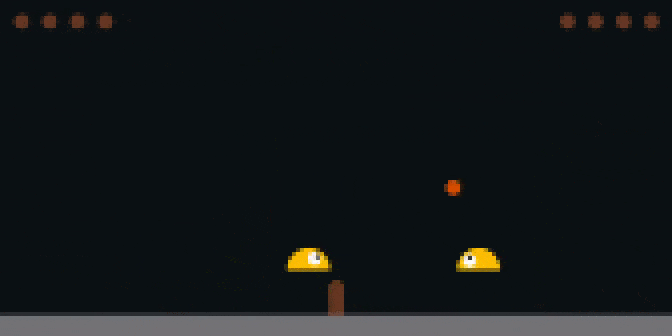
\includegraphics[width=0.8\textwidth]{img/slimevolley.png}
\end{figure}


\begin{figure}[h]
    \caption{Screenshot of Cartpole-swingup environment}
    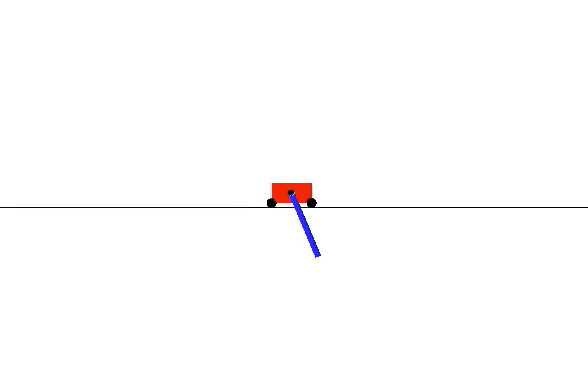
\includegraphics[width=0.8\textwidth]{img/cartpole.png}
\end{figure}

